% Copyright 2018-2019 Melvin Eloy Irizarry-Gelpí
\setcounter{chapter}{10}
\chapter{Simple Harmonic Motion}
%
In this experiment you will study simple harmonic motion.
%
\section{Preliminary}
%
Simple harmonic motion provides a great opportunity to test many important physical laws, some of which you have already seen in previous experiments.
%
\subsection{Hooke's Law}
%
When an elastic spring is stretched or compressed beyond its natural relaxed length, a restorative force arises on the spring that causes the spring to return to its natural relaxed length. This force is proportional to how much distance $x$ the spring is stretched:
\begin{equation} \label{eq.11.hooke}
    F_{k} = - k x
\end{equation}
This relation is known as \textbf{Hooke's law}. Here the minus sign is due to the restorative nature of the force (it is always opposite to what the spring is doing), and $k$ is the \textbf{spring constant}. If force is in newtons (N) and distance from equilibrium is in meters (m), then the spring constant has units of newton-per-meter (N/m).
%
\subsection{Newton's Second Law}
%
If a mass $m$ is attached to one end of the spring, the mass will move back-and-forth when the spring is stretched or compressed. In the absence of other forces, the net force on the object is just the force from the spring.
\begin{equation}
    F_{\text{net}} = F_{k} = -kx
\end{equation}
Due to Newton's second law, you have a relation between \textbf{force} and \textbf{acceleration}:
\begin{equation}
    F_{\text{net}} = m a
\end{equation}
Thus
\begin{equation}
    ma = -kx
\end{equation}
Or in other words:
\begin{equation}
    a = -\left( \frac{k}{m} \right) x
    \label{eq.11.ax}
\end{equation}
That is, for this back-and-forth motion, the acceleration is proportional to the amount of distance that the spring is stretched or compressed. Note that the slope is negative. If $k$ is in N/m, and $m$ is in kg, then $k/m$ will be in N / (kg m), or equivalently:
\begin{equation}
    1 \frac{\text{N}}{\text{kg m}} = 1 \frac{1}{\text{s}^{2}}
\end{equation}
Hence, the slope of the $a$ versus $x$ relation should have units of inverse square time. For convenience, you can introduce
\begin{equation}
    \omega = \sqrt{\frac{k}{m}}
\end{equation}
such that
\begin{equation}
    a = - \omega^{2} x
    \label{eq:11.axomega}
\end{equation}
The physical meaning of $\omega$ will become clear later.
%
\subsection{Sine and Cosine}
%
The \textbf{sine} and \textbf{cosine} functions are very important (and relevant) for simple harmonic motion. These functions are familiar from trigonometry where they are used to express the ratio of lengths in a right triangle.

Figure \ref{figure:11.sin.cos} shows the shape of the cosine and sine functions. These functions oscillate between $\pm 1$ and are \textbf{periodic}. More specifically, the horizontal distance between consecutive peaks of $\sin(x)$ and $\cos(x)$ is $2\pi$. Note that the ``angle'' in Figure \ref{figure:11.sin.cos} is not in degrees, but in a system of units known as \textbf{radians}. Most calculators and computers assume that the $x$ is in radians before computing sine or cosine. The conversion factor between radians and degrees is
\begin{equation}
    180 \text{ degrees} = \pi \text{ radians}
\end{equation}
The symbol for radians is rad. For all practical purposes, a radian is equivalent to a pure number without units.
%
\subsection{Sinusoidal Motion}
%
When you look at the position of the object as it changes with time, you will notice a pattern similar to a sine or cosine function. This suggest a \textbf{sinusoidal fit} for position $x$ as a function of time $t$:
\begin{equation}
    x(t) = A_{x} \sin\left( B_{x}t + C_{x} \right) + D_{x}
\end{equation}
Here $A_{x}$ is the position \textbf{amplitude} of the motion (in meters), $B_{x}$ is the position \textbf{angular frequency} (in radians-per-second), $C_{x}$ is the position \textbf{phase shift} (in radians), and $D_{x}$ is the \textbf{position shift} (in meters).

Velocity is defined as the rate of change of position with respect to time. With calculus, this is equivalent to taking a derivative of position with respect to time:
\begin{equation}
    v(t) = \frac{\mathrm{d} x}{\mathrm{d} t} = A_{x}B_{x} \cos\left( B_{x}t + C_{x} \right)
    \label{eq.11.v}
\end{equation}
That is, the fit parameters that describe the sinusoidal fit for position (i.e. $A_{x}$, $B_{x}$, $C_{x}$, and $D_{x}$) can also be used to describe the sinusoidal fit for velocity.

Similarly, acceleration is defined as the rate of change of velocity with respect to time. With calculus, this is equivalent to taking a derivative of velocity with respect to time:
\begin{equation}
    a(t) = \frac{\mathrm{d} v}{\mathrm{d} t} = -A_{x}B^{2}_{x} \sin\left( B_{x}t + C_{x} \right)
    \label{eq.11.a}
\end{equation}
Again, the parameters that describe the sinusoidal fit for position can also be used to describe the sinusoidal fit for acceleration.

As observed during the experiment, the amount of force over time also has a pattern similar to a sine or cosine function. Since force and position are different physical quantities, some of the fit parameters will have different units:
\begin{equation}
    F(t) = A_{F} \sin\left(B_{F} t + C_{F}\right) + D_{F}
\end{equation}
Here $A_{F}$ is the force \textbf{amplitude} (in newtons), $B_{F}$ is the force \textbf{angular frequency} (in radians-per-second), $C_{F}$ is the force \textbf{phase shift} (in radians), and $D_{F}$ is the \textbf{force shift} (in newtons).

Based on Hooke's law, you would expect some relations between the fit parameters of force and position:
\begin{equation}
    F(t) = - k x(t)
\end{equation}
This relation gives
\begin{equation}
    A_{F} \sin\left(B_{F} t + C_{F}\right) + D_{F} = -k A_{x} \sin\left( B_{x}t + C_{x} \right) - kD_{x}
\end{equation}
That is, you expect
\begin{align}
    A_{F} = kA_{x} && B_{F} = B_{x} && \vert C_{F} - C_{x} \vert = \pi && D_{F} = -kD_{x}
\end{align}
Since force and position are being measured by different sensors, these relations are non-trivial.
%
\subsection{Period of Oscillation and Angular Frequency}
%
For a mass $m$ attached to a spring with spring constant $k$, the \textbf{period of oscillation} is given by
\begin{equation}
    T = 2\pi \sqrt{\frac{m}{k}}
\end{equation}
The period is the time it takes for the mass to do one full cycle. Related to the period is the \textbf{angular frequency} $\omega$:
\begin{equation}
    \omega = \frac{2 \pi}{T} = \sqrt{\frac{k}{m}}
    \label{eq.11.omega}
\end{equation}
You have already seen the appearance of $\omega^{2}$ as the slope in the $a$ versus $x$ relation in Figure \ref{eq:11.axomega}. As you are going to see, the same value of angular frequency controls how quickly position, velocity, acceleration, and force change with time.
%
\section{Experiment}
%
You used a motion sensor to measure the position, velocity and acceleration of a mass hanging from a spring. The spring in turn hangs from a force sensor that you used to measure force. If the sensor is zeroed correctly, the constant weight force $mg$ is taken into account. When the hanging mass is moved from equilibrium and released, the motion was oscillatory.

After recording data for a short time, you used the LabQuest device to obtain the values of the fit parameters that best describe both the force and the position data versus time.

You used four combinations of mass and spring constant, as stated in Table \ref{table.11.parameters}.
%
\section{Analysis}
%
There are many aspects of simple harmonic motion that can be verified with this experiment.
%
\subsection{Force and Position}
%
You can verify \textbf{Hooke's law}, equation (\ref{eq.11.hooke}), by making a scatter chart with \textbf{position} in the horizontal axis, and \textbf{force} in the vertical axis. The shape of this chart should be a downward line, as in Figure \ref{figure.11.hooke}. You can find the slope with the \texttt{SLOPE} function. If position is in column \texttt{X} with the first value in row \texttt{6}, and force is in column \texttt{Y}, with first value in row \texttt{6}; then the command is
\begin{equation}
    \texttt{=SLOPE(Y6:Y, X6:X)}
\end{equation}
The linear behavior confirms Hooke's law. The slope of the linear fit corresponds to the (negative) value of the \textbf{spring constant}. Conversely, the negative of the slope serves as an indirect measurement of the spring constant:
\begin{equation}
    k_{\text{obs}} = - (\text{slope of force versus position linear fit})
\end{equation}
Note that position and force data come from \textbf{different} sensors.
%
\subsection{Force and Acceleration}
%
You can verify \textbf{Newton's second law of motion} by making a scatter chart with \textbf{acceleration} in the horizontal axis, and \textbf{force} in the vertical axis. The shape of this chart should be an upward line, as in Figure \ref{figure.11.newton}. You can find the slope with the \texttt{SLOPE} function. The linear behavior confirms Newton's second law, and the value of the slope is \textbf{mass}. You can use this slope as an indirect measurement of the amount of mass hanging from the spring:
\begin{equation}
    m_{\text{obs}} = \text{slope of force versus acceleration linear fit}
\end{equation}
Note that acceleration and force data come from \textbf{different} sensors.

Together with the measurement of the spring constant from the force versus position chart, you can compute an experimental estimate of the angular frequency via
\begin{equation}
    \omega_{1} = \sqrt{\frac{k_{\text{obs}}}{m_{\text{obs}}}}
\end{equation}
%
\subsection{Acceleration and Position}
%
Combining Hooke's law with Newton's second law of motion gives equation (\ref{eq.11.ax}). Using the definition of $\omega$ in equation (\ref{eq.11.omega}), we find that indeed,
\begin{equation}
    a = -\omega^{2}x
\end{equation}
That is, for simple harmonic motion, the acceleration is proportional to the position with the slope being the (negative) square angular frequency. The shape of this chart should be a downward line, as in Figure \ref{figure.11.ax}. The slope of this chart should be the negative of the squared angular frequency. This value provides another experimental estimate of the angular frequency:
\begin{equation}
    \omega_{2} = \sqrt{- (\text{slope of acceleration versus position})}
\end{equation}
%
\subsection{Common Angular Frequency}
%
From the LabQuest device, you obtained the parameters for the sinusoidal fit for both position and force. Both the $B_{x}$ parameter in the position fit, and the $B_{F}$ parameter in the force fit should correspond to the angular frequency of the simple harmonic motion. Hence, the $B_{x}$ parameter in the position fit provides another experimental estimate of the angular frequency:
\begin{equation}
    \omega_{3} = B_{x} \text{ from position fit}
\end{equation}
and the $B_{F}$ parameter from the force fit provides another experimental estimate of the angular frequency:
\begin{equation}
    \omega_{4} = B_{F} \text{ from force fit}
\end{equation}
Note that, since the data for position and force comes from different sensors, these measurements can be taken as fully independent.

In principle you can perform a sinusoidal fit on velocity and acceleration too. However, the parameters of these fits are not independent. Indeed, theoretically, they depend on the parameters for the position fit as stated in equations (\ref{eq.11.v}) and (\ref{eq.11.a}).
%
\subsection{Velocity and Position}
%
A chart with velocity and position is called a \textbf{phase space} chart. For this particular experiment with simple harmonic motion, the velocity and position data yield an \textbf{elliptical shape} (a closed orbit), as in Figure \ref{figure.11.phase}. Now you know!
%
\section{My Data}
%
My data consist of 12 runs:
\begin{itemize}
    \item Runs 1, 2, and 3: $k = 5$ N/m and $m = 50$ g.
    \item Runs 4, 5, and 6: $k = 5$ N/m and $m = 100$ g.
    \item Runs 7, 8, and 9: $k = 15$ N/m and $m = 150$ g.
    \item Runs 10, 11, and 12: $k = 15$ N/m and $m = 200$ g.
\end{itemize}
Table \ref{table.11.fit} summarizes the sinusoidal fit parameters for the position and force data. Table \ref{table.11.k.m} summarizes the experimental estimates for the spring constant and the mass. Table \ref{table.11.omega} summarizes the results for all the estimates of the angular frequency.
%
\section{Your Data}
%
You should have considered four distinct combinations of spring constant and mass, and taken at least three runs for each combination.
%
\newpage
\section{Your Laboratory Report}
%
In your lab report you should include:
\begin{itemize}
    \item One table like Table \ref{table.11.fit} with the fit parameters. Also include a column with the values for $\vert C_{F} - C_{x} \vert$, and a column with the values for $A_{F} / A_{x}$.
    \item One table like Table \ref{table.11.k.m} with the observed values for the spring constant and mass.
    \item One table like Table \ref{table.11.omega} with all the estimates of the angular frequency. Include a column with the average value, and a column with the percent difference of the average value and the expected value.
    \item One force versus position chart with the linear fit, for a run of your choosing. See Figure \ref{figure.11.hooke}.
    \item One force versus acceleration chart with the linear fit, for a run of your choosing. See Figure \ref{figure.11.newton}.
    \item One acceleration versus position chart with the linear fit, for a run of your choosing. See Figure \ref{figure.11.ax}.
    \item One velocity versus position chart for a run of your choosing. See Figure \ref{figure.11.phase}.
\end{itemize}
You should answer the following questions:
\begin{enumerate}
    \item Based on your analysis and what we saw in class, are you convinced that (for simple harmonic motion) position, velocity, acceleration, and force can all be described by sines or cosines with a common angular frequency?
    \item Is the angular frequency parameter $B_{x}$ for the position versus time chart the same or close to the angular frequency parameter $B_{F}$ for the force versus time graph?
    \item Can you test Newton's second law with the data from this experiment? Does the measured mass agree with the expected value used?
    \item Can you test Hooke's law with the data from this experiment? Does the measured spring constant agree with the expected value used?
    \item Are your four estimates of the angular frequencies close to the expected theoretical value given by (\ref{eq.11.omega}).
\end{enumerate}
%
\newpage
\section{Tables}
%
\begin{table}[ht]
    \centering
    \begin{tabular}{|r|r|r|}\hline
        $k$ (N/m) & $m$ (kg) & $\omega$ (rad/s) \\ \hline
        5 & 0.05 & 10 \\
        5 & 0.1 & 7.071 \\
        15 & 0.15 & 10 \\
        15 & 0.2 & 8.660 \\
        \hline
    \end{tabular}
    \caption{Four combinations of mass and spring constant, along with the expected $\omega$ value}
    \label{table.11.parameters}
\end{table}
%
\begin{table}[ht]
    \centering
    \begin{tabular}{|l|r|r|r|r|r|r|r|r|}
        \hline
        Units & N & rad/s & rad & m & rad/s & rad & rad & N/m \\
        \hline
        Run & $A_{F}$ & $B_{F}$ & $C_{F}$ & $A_{x}$ & $B_{x}$ & $C_{x}$ & $\vert C_{F} - C_{x} \vert$ & $A_{F} / A_{x}$ \\
        \hline
        1 & 0.18702 & 10.073 & 2.9623 & 0.035833 & 10.074 & 6.1523 & 3.19 & 5.219 \\
        2 & 0.18432 & 10.08 & 5.3656 & 0.035155 & 10.081 & 2.2804 & 3.0852 & 5.243 \\
        3 & 0.14574 & 10.087 & 1.3107 & 0.027684 & 10.087 & 4.5103 & 3.1996 & 5.264 \\
        \hline
        4 & 0.39283 & 7.151 & 1.7351 & 0.074343 & 7.1509 & 4.9147 & 3.1796 & 5.284 \\
        5 & 0.44613 & 7.1512 & 2.0286 & 0.085428 & 7.1476 & 5.2144 & 3.1858 & 5.222 \\
        6 & 0.38923 & 7.1511 & 1.419 & 0.073901 & 7.1519 & 4.5973 & 3.1783 & 5.267 \\
        \hline
        7 & 0.60109 & 10.348 & 0.63061 & 0.035986 & 10.348 & 3.829 & 3.19839 & 16.703 \\
        8 & 0.78886 & 10.341 & 0.65922 & 0.047473 & 10.337 & 3.8649 & 3.20568 & 16.617 \\
        9 & 0.51888 & 10.353 & 0.73697 & 0.030912 & 10.352 & 3.9389 & 3.20193 & 16.786 \\
        \hline
        10 & 0.78128 & 8.9734 & 2.5345 & 0.046803 & 8.9733 & 5.7246 & 3.1901 & 16.693 \\
        11 & 0.89829 & 8.9709 & 3.7414 & 0.053931 & 8.9707 & 0.65011 & 3.09129 & 16.656 \\
        12 & 0.97657 & 8.9683 & 2.5984 & 0.05852 & 8.969 & 5.7868 & 3.1884 & 16.688 \\
        \hline
    \end{tabular}
    \caption{Sinusoidal fit parameters}
    \label{table.11.fit}
\end{table}
%
\begin{table}[ht]
    \centering
    \begin{tabular}{|l|r|r|r|r|}
        \hline
        Units & N/m & kg & N/m & kg \\
        \hline
        Run & Expected $k$ & Expected $m$ & Observed $k$ & Observed $m$ \\
        \hline
        1 & 5 & 0.05 & 5.2038 & 0.0527 \\
        2 & 5 & 0.05 & 5.2371 & 0.0538 \\
        3 & 5 & 0.05 & 5.2618 & 0.0542 \\
        \hline
        4 & 5 & 0.1 & 5.2831 & 0.1061 \\
        5 & 5 & 0.1 & 5.2220 & 0.1041 \\
        6 & 5 & 0.1 & 5.2676 & 0.1056 \\
        \hline
        7 & 15 & 0.15 & 16.6495 & 0.1621 \\
        8 & 15 & 0.15 & 16.5786 & 0.1626 \\
        9 & 15 & 0.15 & 16.7589 & 0.1630 \\
        \hline
        10 & 15 & 0.2 & 16.6761 & 0.2146 \\
        11 & 15 & 0.2 & 16.6199 & 0.2154 \\
        12 & 15 & 0.2 & 16.6586 & 0.2138 \\
        \hline
    \end{tabular}
    \caption{Expected and Observed values for spring constant and mass}
    \label{table.11.k.m}
\end{table}
%
\begin{table}[ht]
    \centering
    \begin{tabular}{|l|r|r|r|r|r|r|r|}
        \hline
        Units & rad/s & rad/s & rad/s & rad/s & rad/s & rad/s & \% \\
        \hline
        Run & Expected $\omega$ & $\omega_{1}$ & $\omega_{2}$ & $\omega_{3}$ & $\omega_{4}$ & Average $\omega$ & P.D. \\
        \hline
        1 & 10.000 & 9.9344 & 9.8570 & 10.073 & 10.074 & 9.9846 & \textminus 0.15\% \\
        2 & 10.000 & 9.8671 & 9.8177 & 10.08 & 10.081 & 9.9615 & \textminus 0.39\% \\
        3 & 10.000 & 9.8499 & 9.7926 & 10.087 & 10.087 & 9.9541 & \textminus 0.46\% \\
        \hline
        4 & 7.071 & 7.0579 & 7.0380 & 7.151 & 7.1509 & 7.0994 & 0.40\% \\
        5 & 7.071 & 7.0825 & 7.0457 & 7.1512 & 7.1476 & 7.1067 & 0.50\% \\
        6 & 7.071 & 7.0626 & 7.0410 & 7.1511 & 7.1519 & 7.1017 & 0.43\% \\
        \hline
        7 & 10.000 & 10.1333 & 10.0744 & 10.348 & 10.348 & 10.2259 & 2.26\% \\
        8 & 10.000 & 10.0982 & 10.0632 & 10.341 & 10.337 & 10.2098 & 2.10\% \\
        9 & 10.000 & 10.1410 & 10.0852 & 10.353 & 10.352 & 10.2328 & 2.33\% \\
        \hline
        10 & 8.660 & 8.8159 & 8.7990 & 8.9734 & 8.9733 & 8.8904 & 2.66\% \\
        11 & 8.660 & 8.7830 & 8.7682 & 8.9709 & 8.9707 & 8.8732 & 2.46\% \\
        12 & 8.660 & 8.8270 & 8.7951 & 8.9683 & 8.969 & 8.8899 & 2.65\% \\
        \hline
    \end{tabular}
    \caption{Experimental estimates of the angular frequency}
    \label{table.11.omega}
\end{table}
%
\FloatBarrier
\newpage
\section{Figures}
%
\begin{figure}[ht]
    \centering
    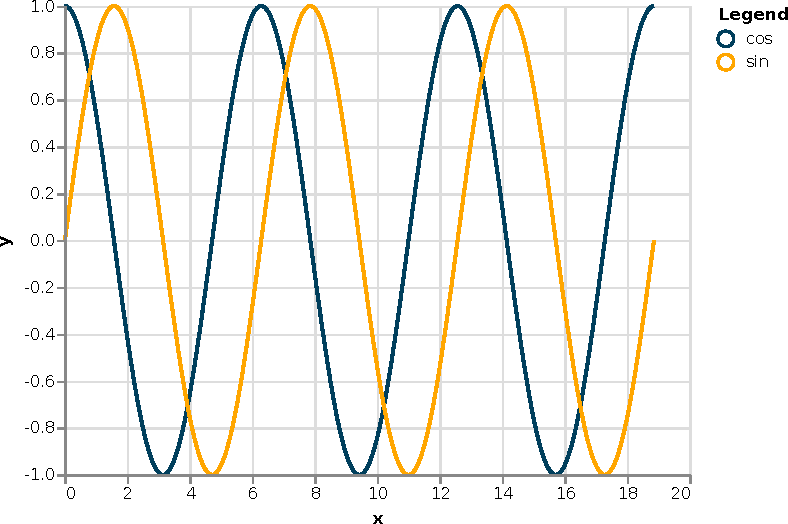
\includegraphics{chart/11-shm/trig.pdf}
    \caption{Sine and Cosine functions}
    \label{figure:11.sin.cos}
\end{figure}
%
\begin{figure}[ht]
    \centering
    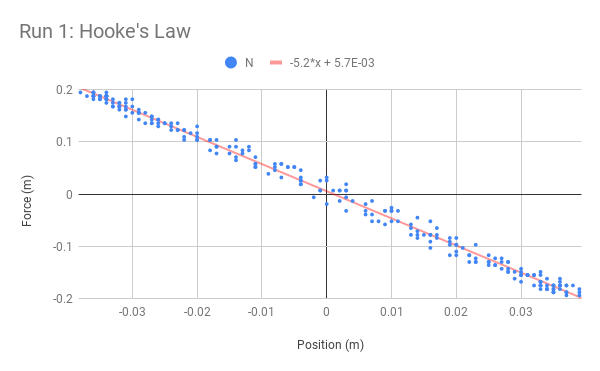
\includegraphics[scale=0.71]{image/11-shm/run-1-hooke.png}
    \caption{Testing Hooke's Law}
    \label{figure.11.hooke}
\end{figure}
%
\begin{figure}[ht]
    \centering
    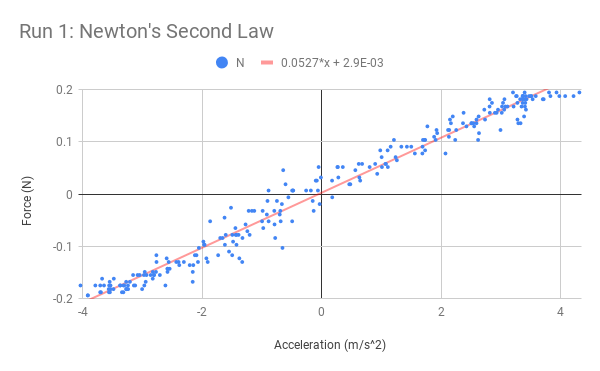
\includegraphics[scale=0.71]{image/11-shm/run-1-newton.png}
    \caption{Testing Newton's Second Law of Motion}
    \label{figure.11.newton}
\end{figure}
%
\begin{figure}[ht]
    \centering
    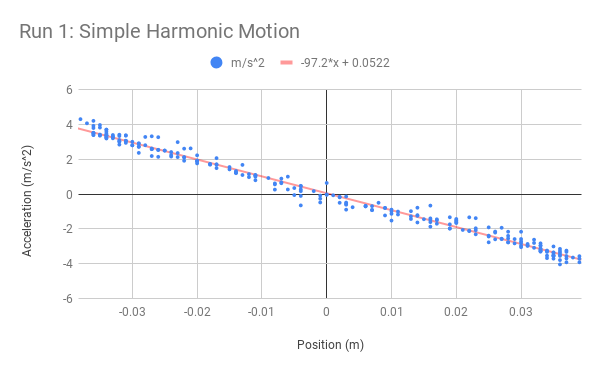
\includegraphics[scale=0.71]{image/11-shm/run-1-shm.png}
    \caption{Testing relation between acceleration and position due to simple harmonic motion}
    \label{figure.11.ax}
\end{figure}
%
\begin{figure}[ht]
    \centering
    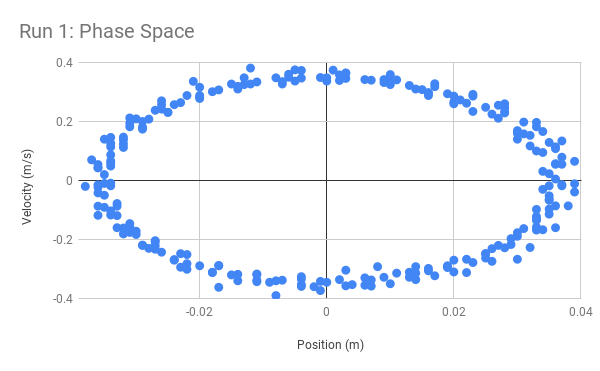
\includegraphics[scale=0.71]{image/11-shm/run-1-phase.png}
    \caption{Visualizing the phase space for simple harmonic motion}
    \label{figure.11.phase}
\end{figure}
%
